\documentclass[11p]{article}
% Packages
\usepackage{amsmath}
\usepackage{graphicx}
\usepackage{fancyheadings}
\usepackage[swedish]{babel}
\usepackage[
    backend=biber,
    style=authoryear-ibid,
    sorting=ynt
]{biblatex}
\usepackage[utf8]{inputenc}
\usepackage[T1]{fontenc}
%Källor
\addbibresource{references.bib}
\graphicspath{ {./images/} }

% Lite variabler
\def\email{Fabian.Sigfridsson@ga.ntig.se}
\def\foottitle{Bakgrund}
\def\name{Fabian Sigfridsson}

\title{Bakgrund \\ \small Gymnasiearbete}
\author{\name}
\date{\today}

\begin{document}

% fixar sidfot
\lfoot{\footnotesize{\name \\ \email}}
\rfoot{\footnotesize{\today}}
\lhead{\sc\footnotesize\foottitle}
\rhead{\nouppercase{\sc\footnotesize\leftmark}}
\pagestyle{fancy}
\renewcommand{\headrulewidth}{0.2pt}
\renewcommand{\footrulewidth}{0.2pt}

% i Sverige har vi normalt inget indrag vid nytt stycke
\setlength{\parindent}{0pt}
% men däremot lite mellanrum
\setlength{\parskip}{10pt}

\maketitle

\section{Referenser}


Referenser i text kan skrivas på två sätt: Enligt \textcite{} kan man använde två typer av referenser, inbäddade i texten eller ``efter'' ett fakta \parencite{Fraenkel}. Ett till test för att se hur det ser ut \parencite{fermi}.

\section{Annat som kan vara bra att veta}
Det är lätt att skriva matematik i \LaTeX

\begin{equation}
    F = G \frac{M m}{r^2}
    \label{eq:grav}
\end{equation}

Ekvation \eqref{eq:grav} känner ni igen...
\clearpage
\subsection{En underrubrik}
    \begin{figure}[!h]
        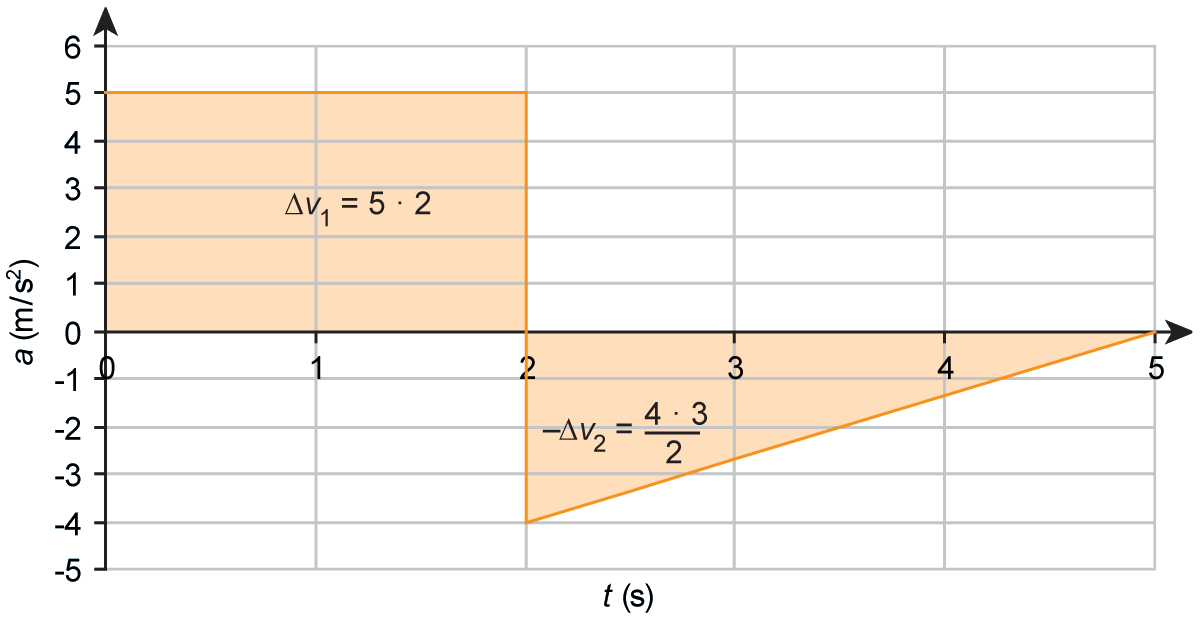
\includegraphics[width=0.8\textwidth]{accelerationTime.png}
        \caption{Acceleration-tid diagram. Källa: \textcite{Fraenkel}}
        \label{fig:acc}
    \end{figure}

Acceleration-tiddiagram (se figur \ref{fig:acc})

\printbibliography

\end{document}
